\newpage

\section{Введение}

\vspace{0.5cm}
\hspace{0.6cm}
В рамках производстенной практики необходимо было реализовать базу данных на MS SQL со связкой с C Sharp. 

\section{Сфера деятельности компании}

\vspace{0.5cm}
\hspace{0.6cm}
Компания «Цезарь Сателлит» - ведущий оператор систем безопасности для автомобилей и недвижимости.

\vspace{0.1cm}
Группа компаний «Цезарь Сателлит», созданная в 2000 году, является основателем и ключевым поставщиком рынка телематических услуг и комплексной безопасности на территории России. Более 200 000 частных клиентов и собственников бизнеса доверили компании самое дорогое: личную безопасность, защиту автомобиля, дома и офиса.

\vspace{0.1cm}
Использование новейших спутниковых (ГЛОНАСС/GPS) и мобильных (GSM) технологий, собственные патентованные разработки, развитая мониторинговая инфраструктура, уникальные технологии розыска и тесное взаимодействие с полицией – все это позволяет компании идти на опережение и противостоять современным методам угона.

\vspace{0.1cm}
«Цезарь Сателлит» сегодня – это 20 лет на рынке, 3 отказоустойчивых центра безопасности, которые выполняют мониторинг тревожных сигналов в режиме 24/7, самый значительный состав групп быстрого реагирования – более 5 000 собственных и партнерских экипажей, готовых выехать по первому сигналу тревоги.

\vspace{0.1cm}
Клиентами компании являются лидеры автомобильной промышленности, такие как BMW Russland Trading, Toyota Motor, Jaguar Land Rover, Mazda Motor Rus, Ford Sollers и крупнейшие автодилеры по всей стране. Под охраной «Цезарь Сателлит» находится значительная доля банковского сектора (Сбербанк, Райффайзенбанк, Ситибанк, Абсолют банк, Росбанк, БинБанк), ключевые сети розничной торговли (X5 Retail Group, «Азбука вкуса», «Магнит», «Дикси»).

\vspace{0.1cm}
Ежедневно «Цезарь Сателлит» предотвращает десятки случаев краж и автомобильных угонов по всей территории России, в странах Европы, Азии и СНГ, обеспечивая сохранность жизни и имущества своих клиентов\cite{csat}.


\newpage
\section{Основная часть}

\vspace{0.5cm}
\hspace{0.6cm}
Для реализации поставленной задачи была выбрана система управления реляционными базами данных, разработанная копорацие Microsoft, Microsoft SQL Server 2017. Выбор MS SQL 2017 был обусловлен стабильностью работы и совместимостью с языком программирования C Sharp. База данных, написанная на MS SQL, может подключится к C Sharp по прямому подключению, а также по подключению через   фреймворк Entity.



\subsection{Python}

\vspace{0.5cm}
\hspace{0.6cm}
Язык программирования Python использовался для генерации случайных данных для базы данных. Так как заполнение базы данных и придумывание осмысленных данных для ее атрибутов слишком трудозатратная задача, поэтому была выбрана библиотека генерации случайных данных - Faker. С ее помощью было сгенерировано более десяти тысяч строк данных, сравнимых с данными.

\vspace{0.1cm}
Faker - это библиотека Python, которая генерирует поддельные данные. Независимо от того, нужно ли нам загрузить свою базу данных, создать красивые XML-документы, заполнить наш тестотовый сервис, чтобы протестировать его, или анонимизировать данные, взятые из производственной службы.

\begin{lstlisting}[caption=Создание фейковых имен, label = list:pythonFakerName]
	from faker import Faker
	
	fake = Faker()
	
	for _ in range(3):
		print(fake.name())
	
	# 'Elda Palumbo'
	# 'Sig. Alighieri Monti'
	# 'Costanzo Costa'

\end{lstlisting}

\begin{lstlisting}[caption=Генерация фейковых адресов, label = list:pythonFakerAddresses]
	from faker import Faker

	fake = Faker()

	for _ in range(3):
		print(fake.address())

	# Michael Pike Dannyton, AR 20235
	#  Little Wall Apt. 359 East Loretta, NV 16913
	# Steve Park East Austin, MI 06826

\end{lstlisting}


\newpage
\subsection{MS SQL}

\vspace{0.5cm}
\hspace{0.6cm}
На языке SQL было создано две базы данных, предназначенных для оперативного взаимодействия всех компонентов компании. Главной таблицой в базе данных CS1 является таблица Contract. Эта таблица связывает все таблицы в двух базах данных. Через эту таблицу можно получить информацию о машинах оперделенного пользователя, какие сообщение приходили на оборудование, устоновленные в этой машине. Также можно определить в каком сервисном центре клиент устанавливал оборудование и когда это оборудование последний раз проверялось.

\vspace{0.1cm}
База данных, представленная на рисунке \ref{img:db_cs} спроектирована и приведена третьей нормальной форме.

\newpage
\begin{figure}[H]
	\centering
	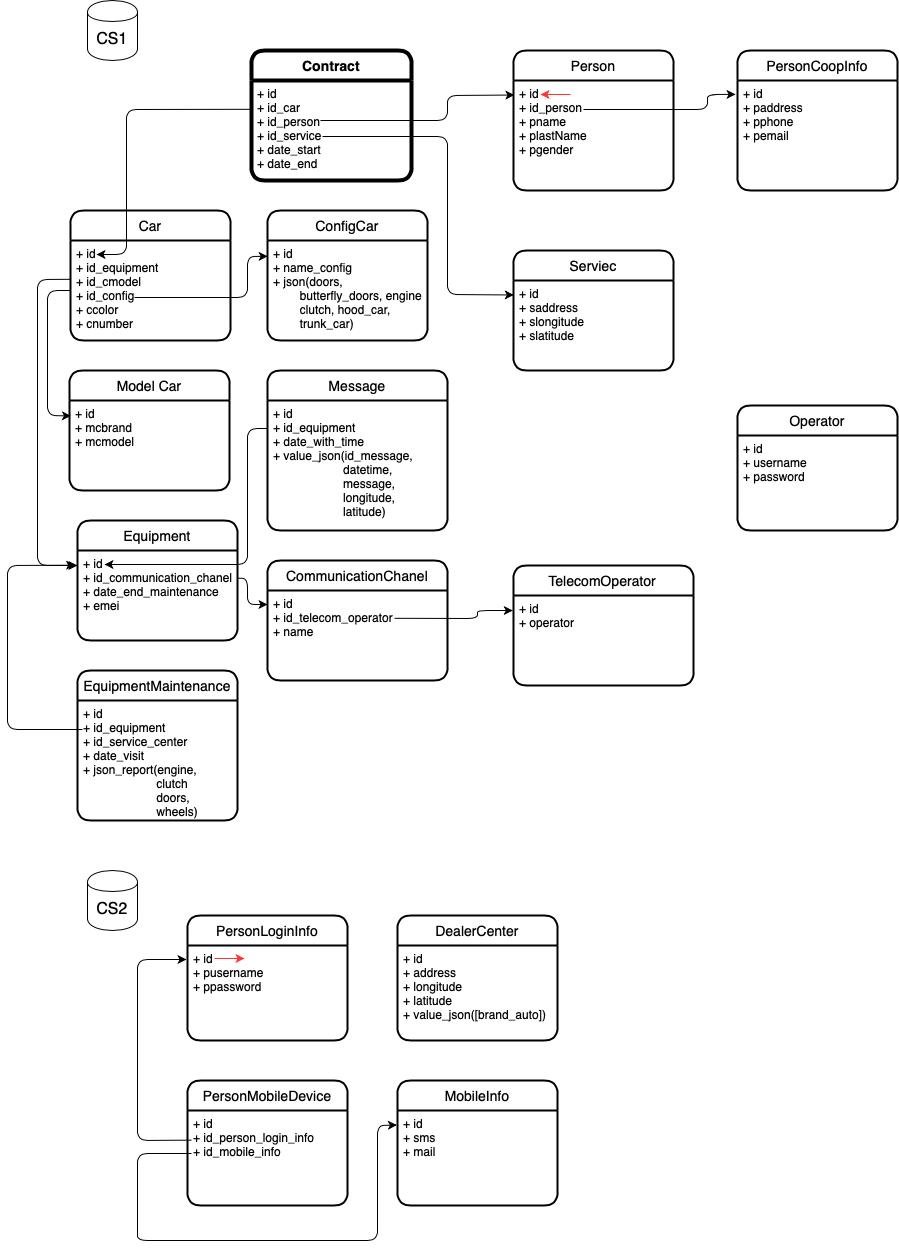
\includegraphics[scale=0.52]{img/bd_cs.png}
	\caption{Спроектированная база данных}
	\label{img:db_cs}
\end{figure}


\newpage
\vspace{0.5cm}
База данных CS1 состоит из следующих таблиц:
\begin{itemize}
	\item \textbf{Contract}- таблица с контрактами пользователей;
	\item \textbf{Person} - таблица с именем и фамилией клиента;
	\item \textbf{PersonCoopInfo} - таблица с контактами, по которым можно связать с клиентами;
	\item \textbf{Serviec} - таблица с адресами сервисов, устанавливающих оборудование компании клиентам;
	\item \textbf{Operator} - таблица с логинами и паролями операторов, мониторящих события, происходящие с имуществом клиентов;
	\item \textbf{Car} - таблица с номером и цветом машины клиента;
	\item \textbf{ConfigCar} - таблица с конфигурацией оборудования, поставленного на конкретную машину;
	\item \textbf{ModelCar} - таблица с брендом и моделью машины клиента;
	\item \textbf{Equipment} -  таблица с информаций об оборудование;
	\item \textbf{EquipmentMaintenance} - таблица с информацией о последнем техническом осмотре оборудования;
	\item \textbf{Message} - таблица с сообщениями, пришедшими на конкретное оборудование;
	\item \textbf{CommunicationChanel} - таблица с каналом коммуникации, установленным в оборудование;
	\item \textbf{TelecomOperator} - таблица с операторами связи.
	
\end{itemize}

\vspace{0.5cm}
База данных CS2 состоит из следующих таблиц:
\begin{itemize}
	\item \textbf{PersonLoginInfo}- таблица с логинами и паролями пользователей, для входа в систему для мониторинга состояния их имущества;
	\item \textbf{PersonMobileDevice}- таблица информацией о включенных функциях на мобильных устройствах;
	\item \textbf{MobileInfo}- таблица с информацией о включенных методах оповещения;
	\item \textbf{DealerCenter}- таблица с информацией о местоположении дилерских центров.
\end{itemize}


\subsection{C Sharp}

\vspace{0.5cm}
\hspace{0.6cm}
С Sharp (произносится как "си шарп") — современный объектно-ориентированный и типобезопасный язык программирования. C Sharp относится к широко известному семейству языков C, и покажется хорошо знакомым любому, кто работал с C, C++, Java или JavaScript.

\vspace{0.1cm}
C Sharp является объектно-ориентированным языком, но поддерживает также и компонентно-ориентированное программирование. Разработка современных приложений все больше тяготеет к созданию программных компонентов в форме автономных и самоописательных пакетов, реализующих отдельные функциональные возможности. Главная особенность таких компонентов в том, что они представляют собой модель программирования со свойствами, методами и событиями. У них есть атрибуты, предоставляющие декларативные сведения о компоненте. Они включают в себя собственную документацию. C Sharp предоставляет языковые конструкции, непосредственно поддерживающие такую концепцию работы. Благодаря этому C Sharp подходит для создания и применения программных компонентов\cite{microsoft-csharp}.

\begin{lstlisting}[caption=Генерация фейковых адресов, label = list:pythonFakerAddresses]
	namespace CS_operator
	{
		public partial class FormAuth : Form
		{
			ControllerFormAuth controller;
			public FormAuth()
			{
				InitializeComponent();
			
				this.controller = new ControllerFormAuth();
			}
		
			private void loginButton_Click(object sender, EventArgs e)
			{
			
				if (controller.IsLogged(usernameTextBox.Text, passwordTextBox.Text))
				{
					this.Hide();
					Form1 nextWindow = new Form1(usernameTextBox.Text, passwordTextBox.Text);
					nextWindow.ShowDialog();
				}
				else
				{
					MessageBox.Show("This operator does not exist");
				}
			}
		}
	}
\end{lstlisting}

\subsection{Windows Forms}

\subsection{Entity Framework}


\newpage
\section{Заключительная часть}

\vspace{0.5cm}
\hspace{0.6cm}
Разработана база данных в связке с десктопным приложением, позволяющим авторизироваться операторам мониторинга и посмотреть всю информацию о клиенте. За время практики база данных приложение для операторов связи было переведено с обычного подключения базы данных к серверу MS SQL на подключение через фреймворк Entity.
